\chapter{Introduction to Smith Chart}\label{lec:lec7}
In the previous lectures, we were able to derive equations for different parameters for a transmission line such as;
\begin{enumerate}[(i)]
\item 	Power delivered to the load
\item	Voltage standing wave ratio (VSWR)
\item	Voltage and current maximum and minimum
\item	Reflection coefficient
\item	Impedance transformation ratio etc.
\end{enumerate}

Up till now, we analyze transmission line characteristics using analytical methods. But in this lecture, we utilize another approach for analyzing the problems of a transmission line which is the \textbf{Graphical Approach}.
This approach involves solving the problems of a transmission line from an image called a \textbf{Smith Chart}.
This approach is most preferred for solving transmission line problems than the analytical approach owing to the following reasons;\\
\begin{enumerate}[(i)]
\item Images have a much longer-lasting impression than equations or text on the human mind.
\item	It is much simpler to use in solving transmission line problems compared to the analytical approach owing to the fact that calculations can be reduced to a significant amount when analyzing the problems of the transmission line.
\item	It is a very compact way of representing the impedance characteristics of transmission lines.

This method if properly understood makes solving transmission line problems much easier and faster.  It can also be used as a means of cross-checking the solution obtained using the analytical method so that one does not go conceptually wrong in solving transmission line problems.
It is very important to understand that the graphical approach does not give the voltage and current solutions but rather it gives the following parameters:
\begin{enumerate}[(i)]
\item	Impedance transformation relationship 
\item Reflection coefficient
\item Voltage standing wave ratio (VSWR)
\item Location of voltage minimum
\item	Location of voltage maximum etc.
\end{enumerate}
\end{enumerate}

This lecture simply develops a basic framework for analyzing the transmission line by graphical approach.
\begin{figure}[h]
\centering
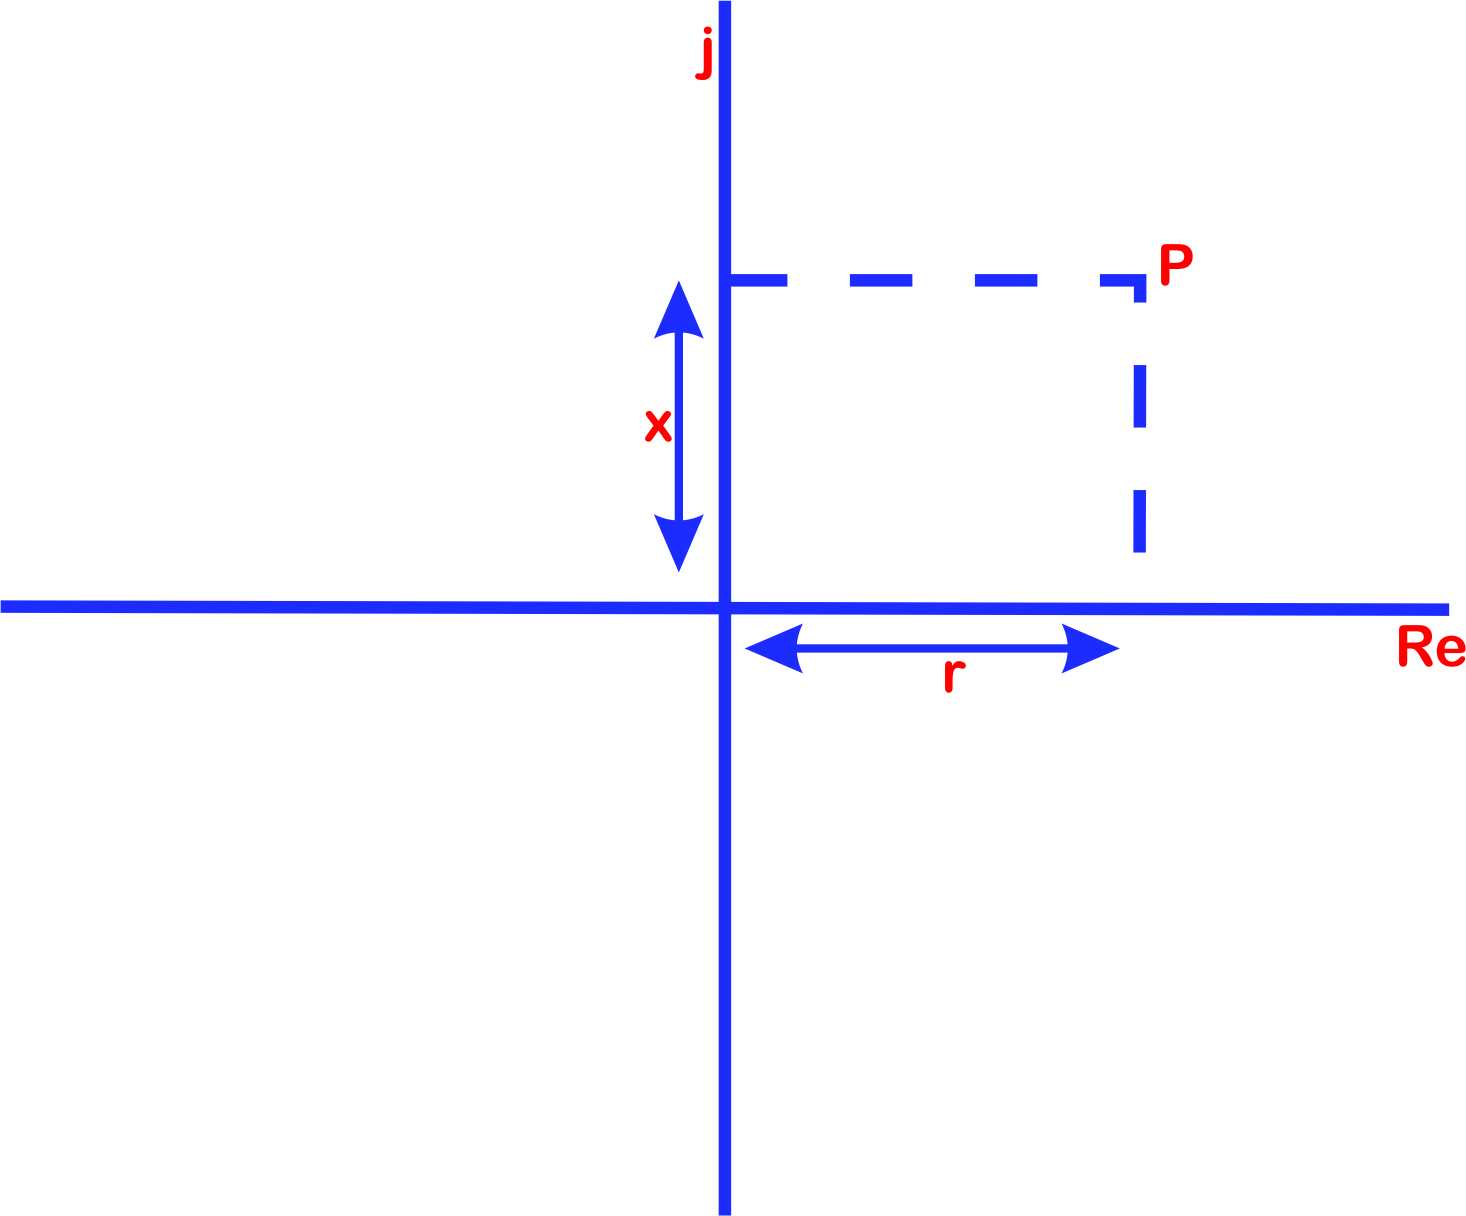
\includegraphics[width=0.5\linewidth]{./graphics/mjhdj}
\caption{Complex Z Plane}
\label{fig:mjhdj}
\end{figure}

\section{Plane Transformation}
It was established in previous lectures that impedances possess a real part and a complex part and this can be written as;
\begin{equation*}
Z= R+jX
\end{equation*}
Where R  represents the real part called Resistance and $jX$ represents the complex part called Reactance. When using the graphical approach, the absolute impedance is not required but instead, normalized impedance is used. It therefore means that, given any impedance, it must be normalized with respect to the characteristic impedance (Zo). i.e
\begin{equation*}
\bar{Z}=\frac{Z_L}{Z_o}
\end{equation*}
where $\bar{Z}$ = normalised impedance\\
$Z_o$ = characteristic impedance\\
$Z_L$   =  absolute  impedance \\
Normalizing the equation above we have: 
\begin{equation*}
\bar{Z}= r + jx
\end{equation*}
Let us represent this expression graphically on a plane which we shall call the impedance plane or Z-plane for short.
\begin{figure}[h]
\center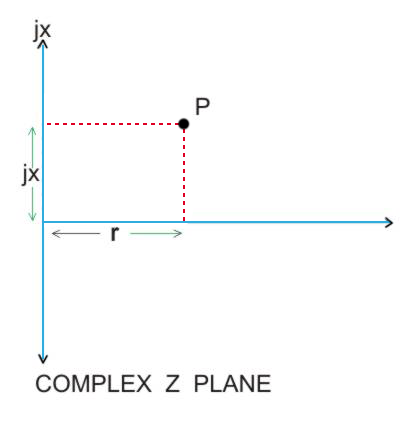
\includegraphics[width=0.5\linewidth]{./graphics/TransLine2 RETOUCHED}
\label{fig:transline2}
\end{figure}

From the figure~\ref{fig:transline2}, it is seen that the resistance r is always real and positive whereas the reactance could be positive which represents Inductive Reactance or negative which represents Capacitive Reactance.\\
Figure~\ref{fig:transline2} represents a possible load which can be obtained from the z-plane.  It can be deduced that all point on the imaginary axis plus all points on the right half plane covers all possible passive loads of a transmission line.
Graphically, the statement is represented in the figure~\ref{fig:oigvbnkliu}
\begin{figure}[h]
\centering
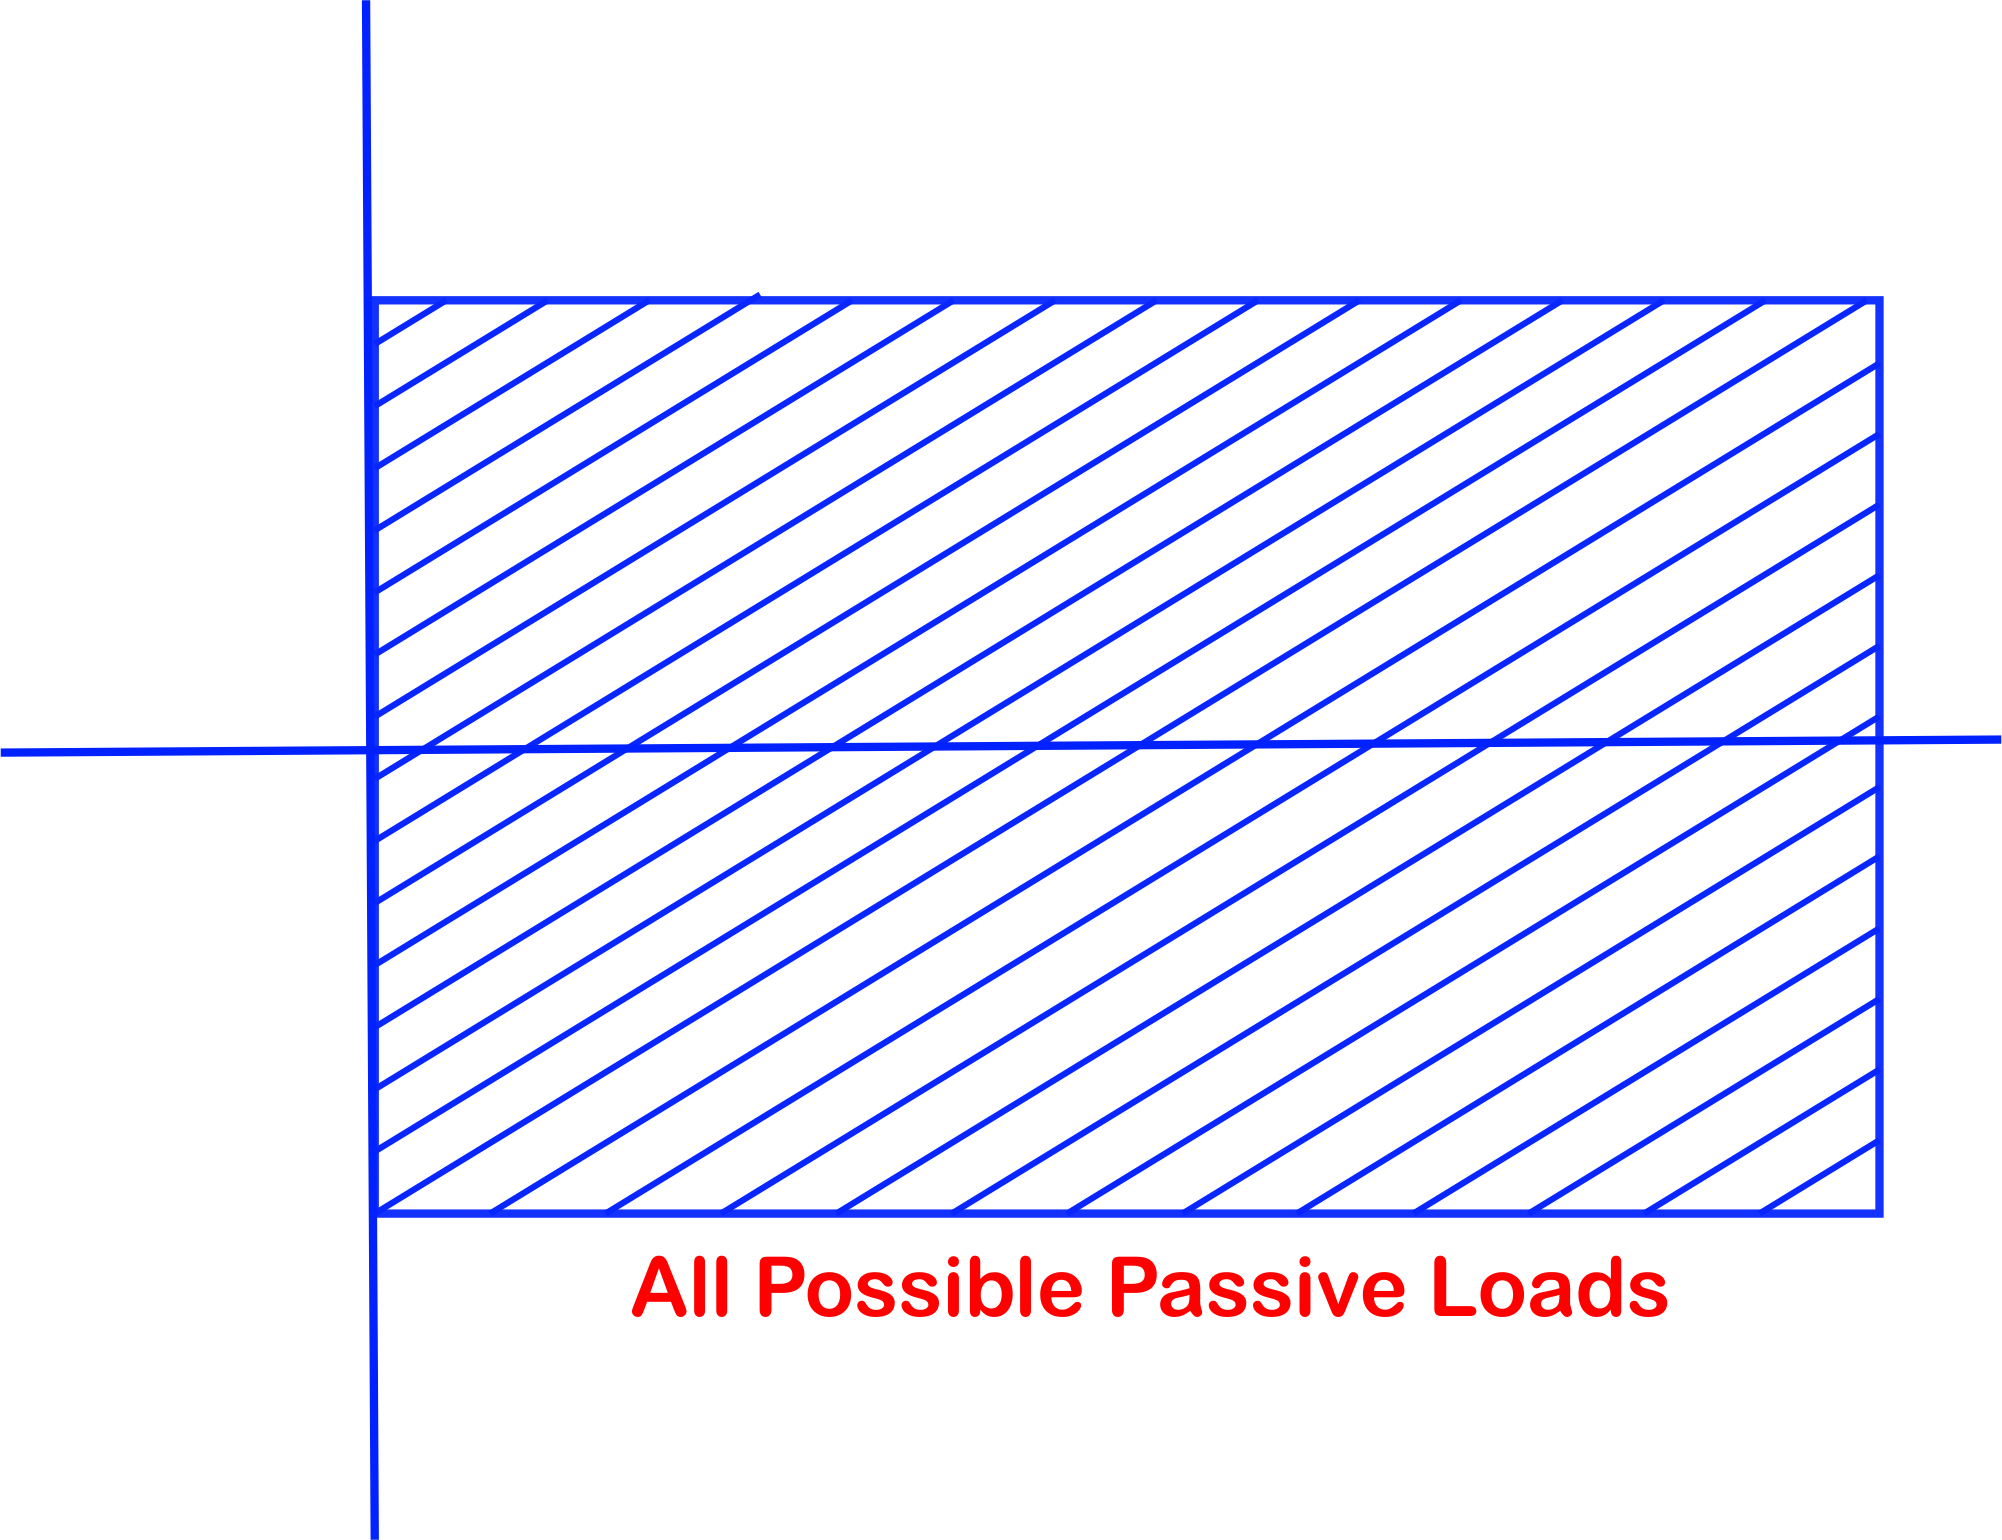
\includegraphics[width=0.6\linewidth]{./graphics/oigvbnkliu}
\caption{All Possible Passive Load}
\label{fig:oigvbnkliu}
\end{figure}

Solving problems of transmission lines using the Z-plane is quite difficult. For this reason, the impedance which was normalized with respect to the characteristic impedance is transformed into another plane which we shall call the Complex Co-efficient Plane or the Gamma Plane ($ \Gamma $).\\ Doing this, expresses the impedances in a form which makes the calculation much simpler.
The transformation from the Z plane to the $ \Gamma $ plane is made possible due to the one-to-one relationship that exists between the impedance Z and the reflection co-efficient $ \Gamma $ i.e
\begin{equation*}
\Gamma = \frac{Z_L - Z_o}{Z_L + Z_o}
\end{equation*}
Normalizing we have
\begin{equation*}
\Gamma= \frac{\bar{Z} - 1}{\bar{Z} + 1}
\end{equation*}\\ or
\begin{equation*}
\bar{Z}= \frac{1 + \Gamma}{1 - \Gamma}
\end{equation*}
This expression simply means if the normalized impedance is known, we can find the reflection coefficient and vice versa.It also means for every value of impedance Z, there is a corresponding value of reflection co-efficient $ \Gamma\ $.\\
Just as Z has real and imaginary parts, $ \Gamma\ $ also has real and imaginary parts which can be written in either rectangular form\\
i.e. $ \Gamma = u + Jv$ or polar form	$\Gamma$ = $Re^{j\theta}$

From previous chapters, it was established that the reflection coefficient for all passive loads is always less than or equal to one($ \Gamma\ \leq 1).$\\
At an open or short circuit, reflection co-efficient $ \Gamma\ $ = 1; for any other impedance $ \Gamma\  < 1$.  So by plotting the reflection co-efficient($ \Gamma\ $) we have the right half Z plane mapping into a unit circle in the gamma plane as shown in figure below.
\begin{figure}[h]
\centering
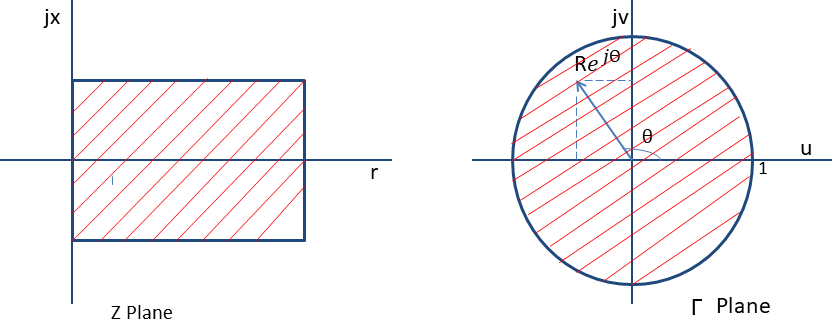
\includegraphics[width=0.7\linewidth]{./graphics/oiuhgvcx}
\caption{Z Plane and Complex $\gamma$ plane}
\label{fig:oiuhgvcx}
\end{figure}

In summary, when solving graphically the problems of transmission lines, the basic idea is to take the impedance which is normalized with respect to the characteristics impedance and do a transformation of this impedance into the gamma plane.

\section{Transformation analysis for complex plane}
\begin{equation}
r + jx =\frac{1 + \Gamma}{1 - \Gamma}
\end{equation}
\begin{equation}
\Gamma\ = u + jv
\end{equation}
substituting 7.3 in 7.2 we have:
\begin{equation}
r + jx = \frac{(1 + u) + jv}{(1 - u) -jv}
\end{equation}
conjugating 7.4 we have:
\begin{equation*}
r + jx = \frac{(1 + u) + jv}{(1 - u) -jv}\times \frac{(1 - u) + jv}{(1 - u) +jv}
\end{equation*}
expanding the expression, we have:
\begin{equation*}
r + jx =\frac{1 - u^2 + jv(1 + u) + jv(1 - u) - v^2}{(1 - u)^2 + jv(1 - u) - jv(1 - u) + v^2} 
\end{equation*}
simplifying the expression, we have:
\begin{equation*}
r + jx = \frac{1 - u^2 + 2jv - v^2}{(1 -u)^2 + v^2}
\end{equation*}
re-arranging the expression
\begin{equation*}
r + jx = \frac{1 - (u^2 + v^2) + 2jv}{(1 - u)^2 + v^2}
\end{equation*}
separating the real and imaginary parts, we have:
\begin{equation}
r = \frac{1 - (u^2 + v^2)}{(1 - u)^2 + v^2}
\end{equation}
and
\begin{equation}
x = \frac{2v}{(1 - u)^2 + v^2}
\end{equation}
considering the real part :	
\begin{equation*}
r = \frac{1 - (u^2 + v^2)}{(1 - u)^2 + v^2}
\end{equation*}
\begin{equation*}
r((1 - u)^2 + v^2) = 1 -(u^2 + v^2)
\end{equation*}
\begin{equation*}
r - 2ur + u^2r + v^2r = 1 - u^2 - v^2
\end{equation*}
collecting like terms, we have:
\begin{equation*}
u^2(r + 1) -2ur + (r - 1) + v^2(r + 1) = 0
\end{equation*}
dividing through by r + 1:
\begin{equation}
u^2 - 2u(\frac{r}{r + 1}) + v^2 +(\frac{r - 1}{r + 1}) = 0
\end{equation}
by using the method of completing the squares:
\begin{align*}
(u - \frac{r}{r+1})^2\;\;+\;\;v^2\;\;+\;\;(\frac{r-1}{r+1})\;\; - \;\;(\frac{r}{r+1})^2\;\; = \;\;0
\end{align*}
\begin{equation*}
(u - \frac{r}{r + 1})^2 + v^2 =(\frac{r}{r + 1})^2 -(\frac{r - 1}{r + 1}) 
\end{equation*}
\begin{equation*}
(u - \frac{r}{r + 1})^2+ v^2 =\frac{r^2 -(r^2 -1)}{(r + 1)^2}
\end{equation*}
\begin{equation}
(u - \frac{r}{r + 1})^2+ v^2 = \frac{1}{(r + 1)^2}
\end{equation}
the expression obtained above represents the equation of a circle in the uv plane centered at$ (\frac{r}{r + 1}, 0) $ with radius $ (\frac{1}{r + 1}) $

equation 7.8 can be compared  with  the equation of a circle of radius r, with origin at x = a and y = 0 which is $ (x - a)^2 + y^2 = r^2 $\\ 
considering the imaginary part, we have:
\begin{equation*}
x =\frac{2v}{(1 - u)^2 + v^2}
\end{equation*}
\begin{equation*}
x(1 - 2u + u^2 + v^2) = 2v
\end{equation*}
\begin{equation*}
v^2x - 2v + u^2x - 2ux + x = 0
\end{equation*}
divide through by x
\begin{equation*}
v^2 - \frac{2v}{x} +u^2 - 2u + 1 = 0
\end{equation*}
factorising the expresssion becomes:
\begin{equation*}
(u - 1)^2 -1 + (v - \frac{1}{x})^2 -\frac{1}{x^2} + 1 = 0
\end{equation*}
\begin{equation}
(u - 1)^2 + (v - \frac{1}{x})^2 = \frac{1}{x^2}\label{eqn:circleuvplane}
\end{equation}
equation~\eqref{eqn:circleuvplane} represents the equation of a circle in the UV plane centred at $ (1,\frac{1}{x}) $ with radius $ (\frac{1}{x}) $.
It can also be compared with the equation of a circle centered at (a,b) and radius r which is $ (x - a)^2 + (y-b)^2 = r^2 $

From the two expressions obtained from solving for r and x,  It can be deduced that for any value of r and x, we gets a circle on the gamma plane. The circle that corresponds to r is called the Circle of Constant Resistance while that corresponds to x is called the Circle of Constant Reactance.

All points on the circle of constant resistance have the same resistance value in the Z plane and all points on the circle of constant reactance will have the same reactance in the Z plane.

\section{Circle of Constant Resistance}
This circle  obtained from the real point of normalized impedance $ \bar{Z} $, the circle lies on the real axis in the gamma plane, and its radius varies from 0 to $\infty$. Plotting the circle for different values of r, we have as shown above;
\begin{figure}[h]
\centering
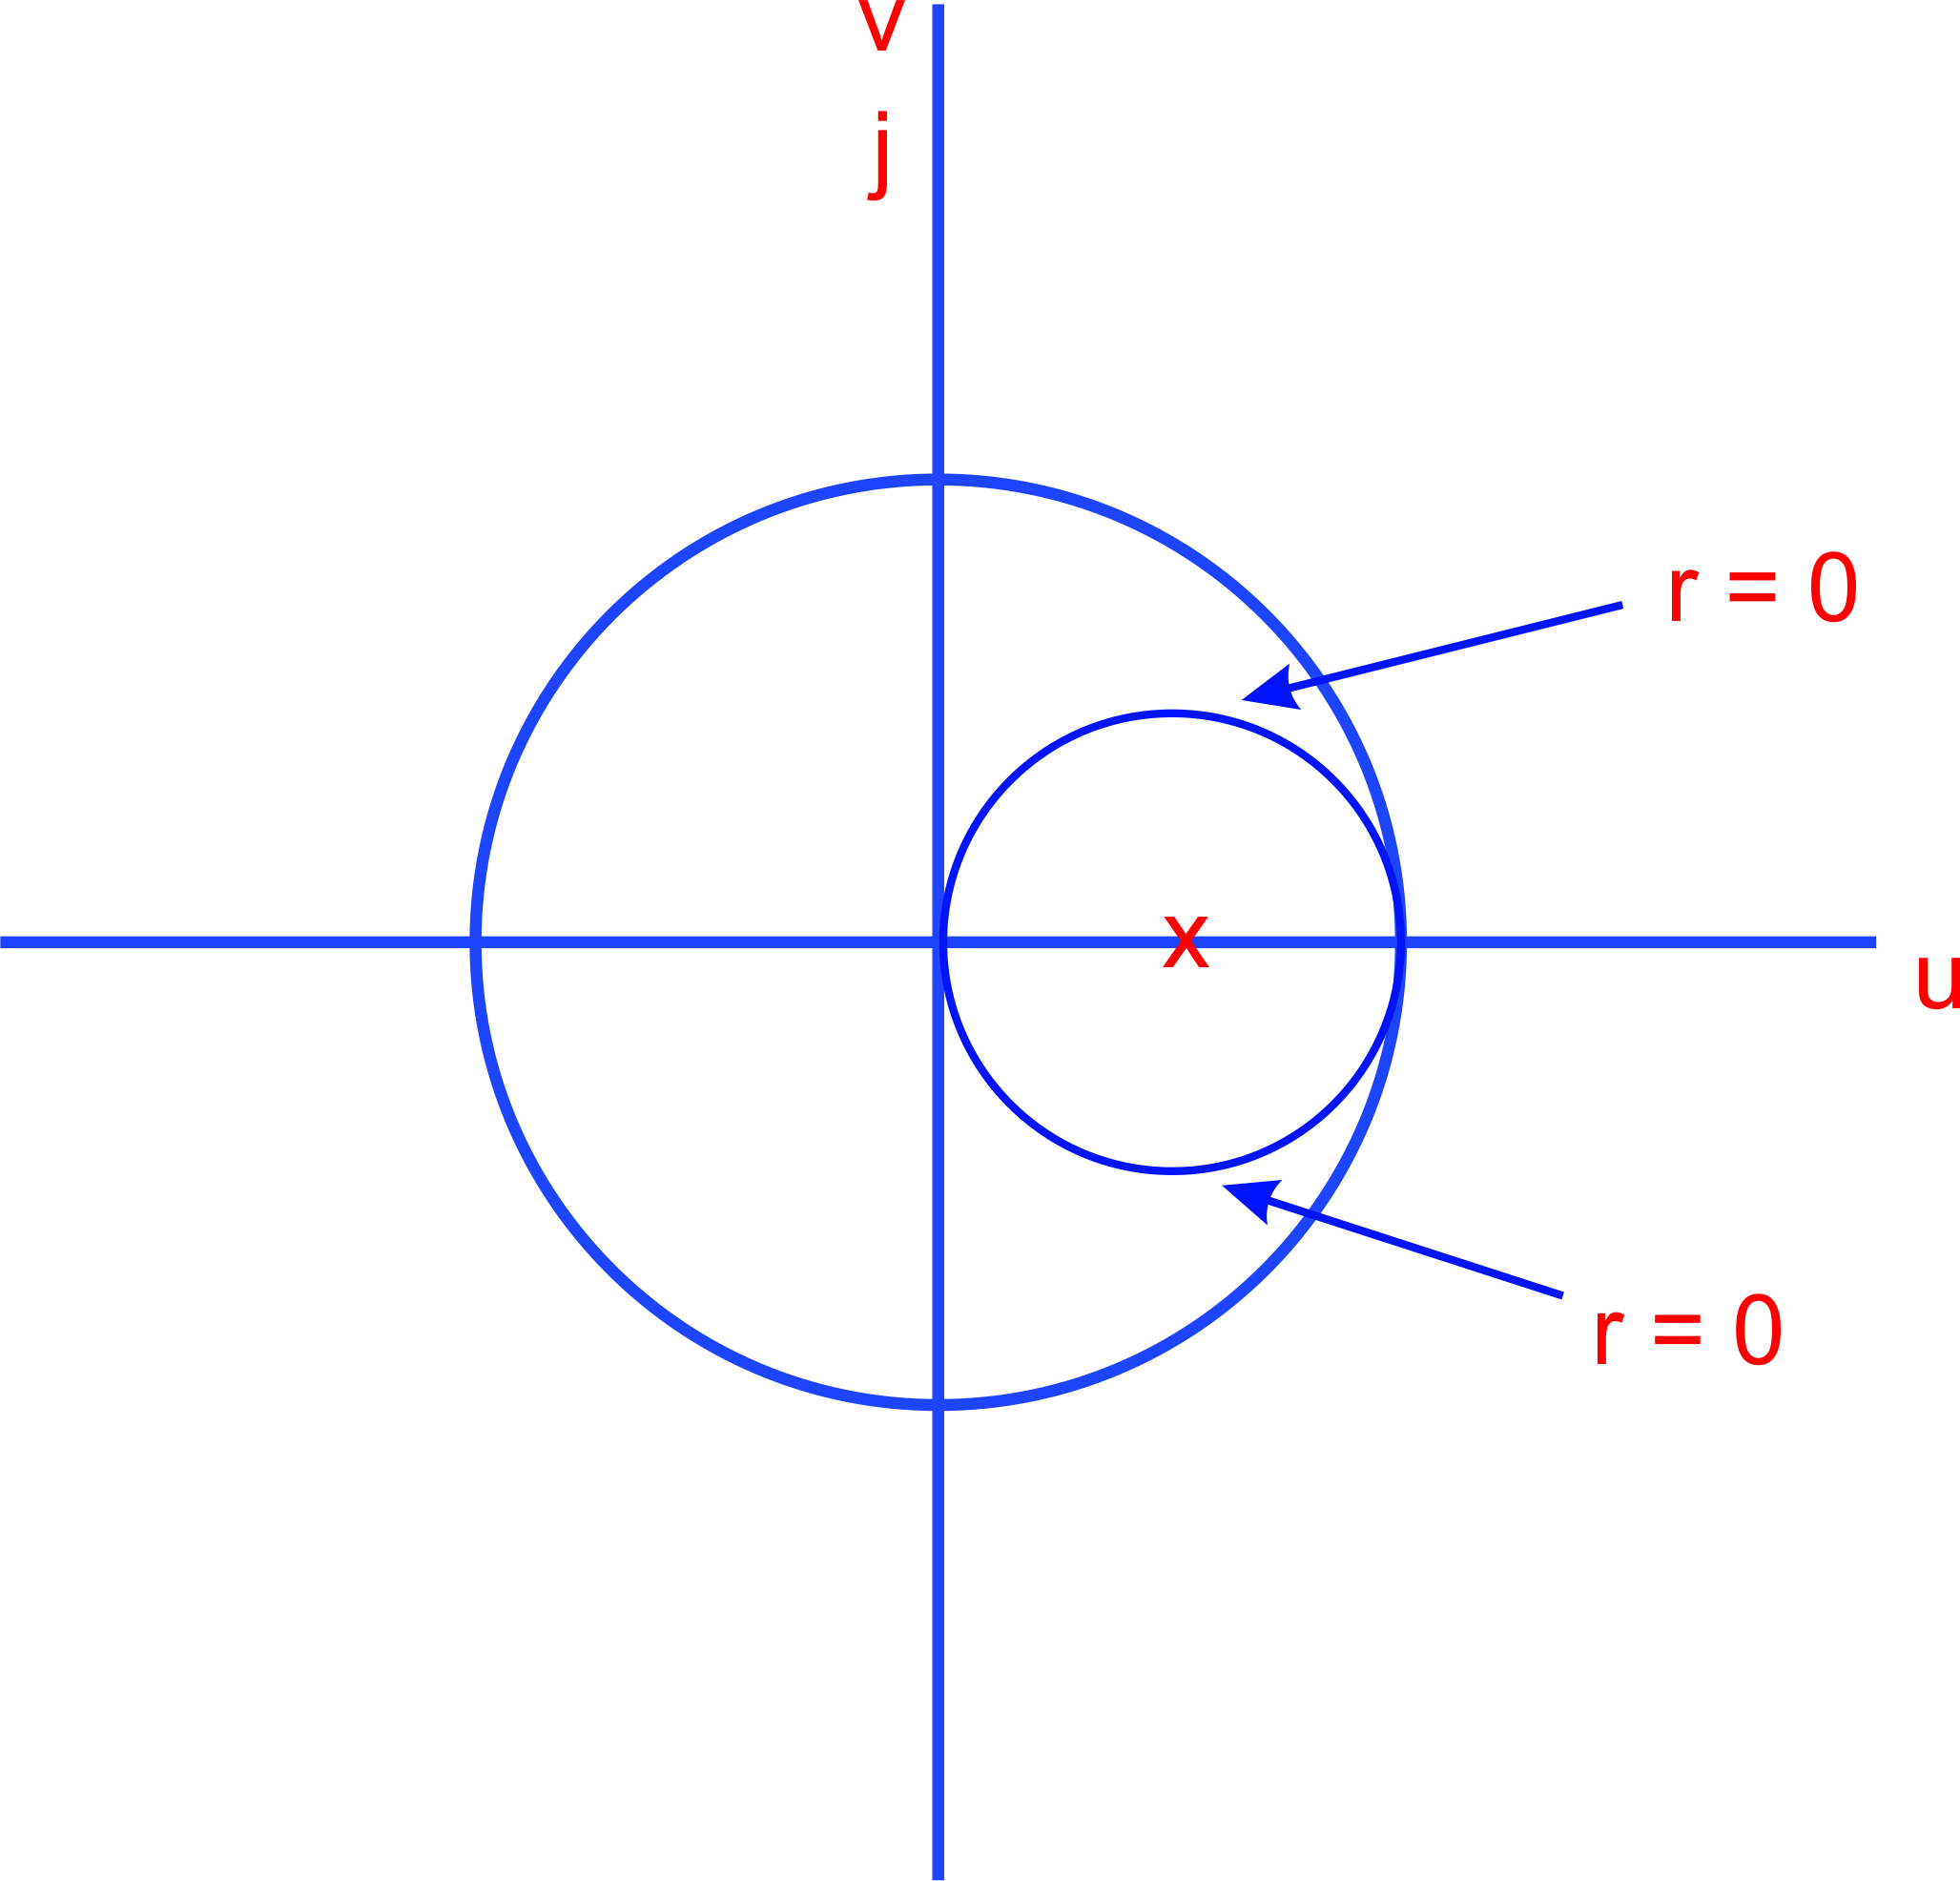
\includegraphics[width=0.5\linewidth]{./graphics/ouytre}
\caption{Circle of Constant Rsistance}
\label{fig:ouytre}
\end{figure}

\begin{equation*}
u^2 - 2u\left(\frac{r}{r + 1}\right) + v^2 +\left(\frac{r - 1}{r + 1}\right) = 0
\end{equation*}
Center = $(\frac{r}{r + 1},0)$ and radius = $\frac{1}{r + 1}$\\\\
Lets plot for various value of r, by varying it from zero to infinity, with r = 0, Center (0,0), and radius = 1.\\
At $r = 1$ which means $Z = Z_o$ we get the centre as $(\dfrac{1}{2}, 0)$ and radius as $\dfrac{1}{2}$.\\
The figure above shows that as the value of r increases, the centre shifts towards the right and the radius keeps reducing towards zero. At $r = \infty$, the centre is (1,0) and the radius is zero, which is denoted as a dot on the real axis. Hence for increasing r, we have the following set of curves.\\\\
\begin{figure}[h]
\centering
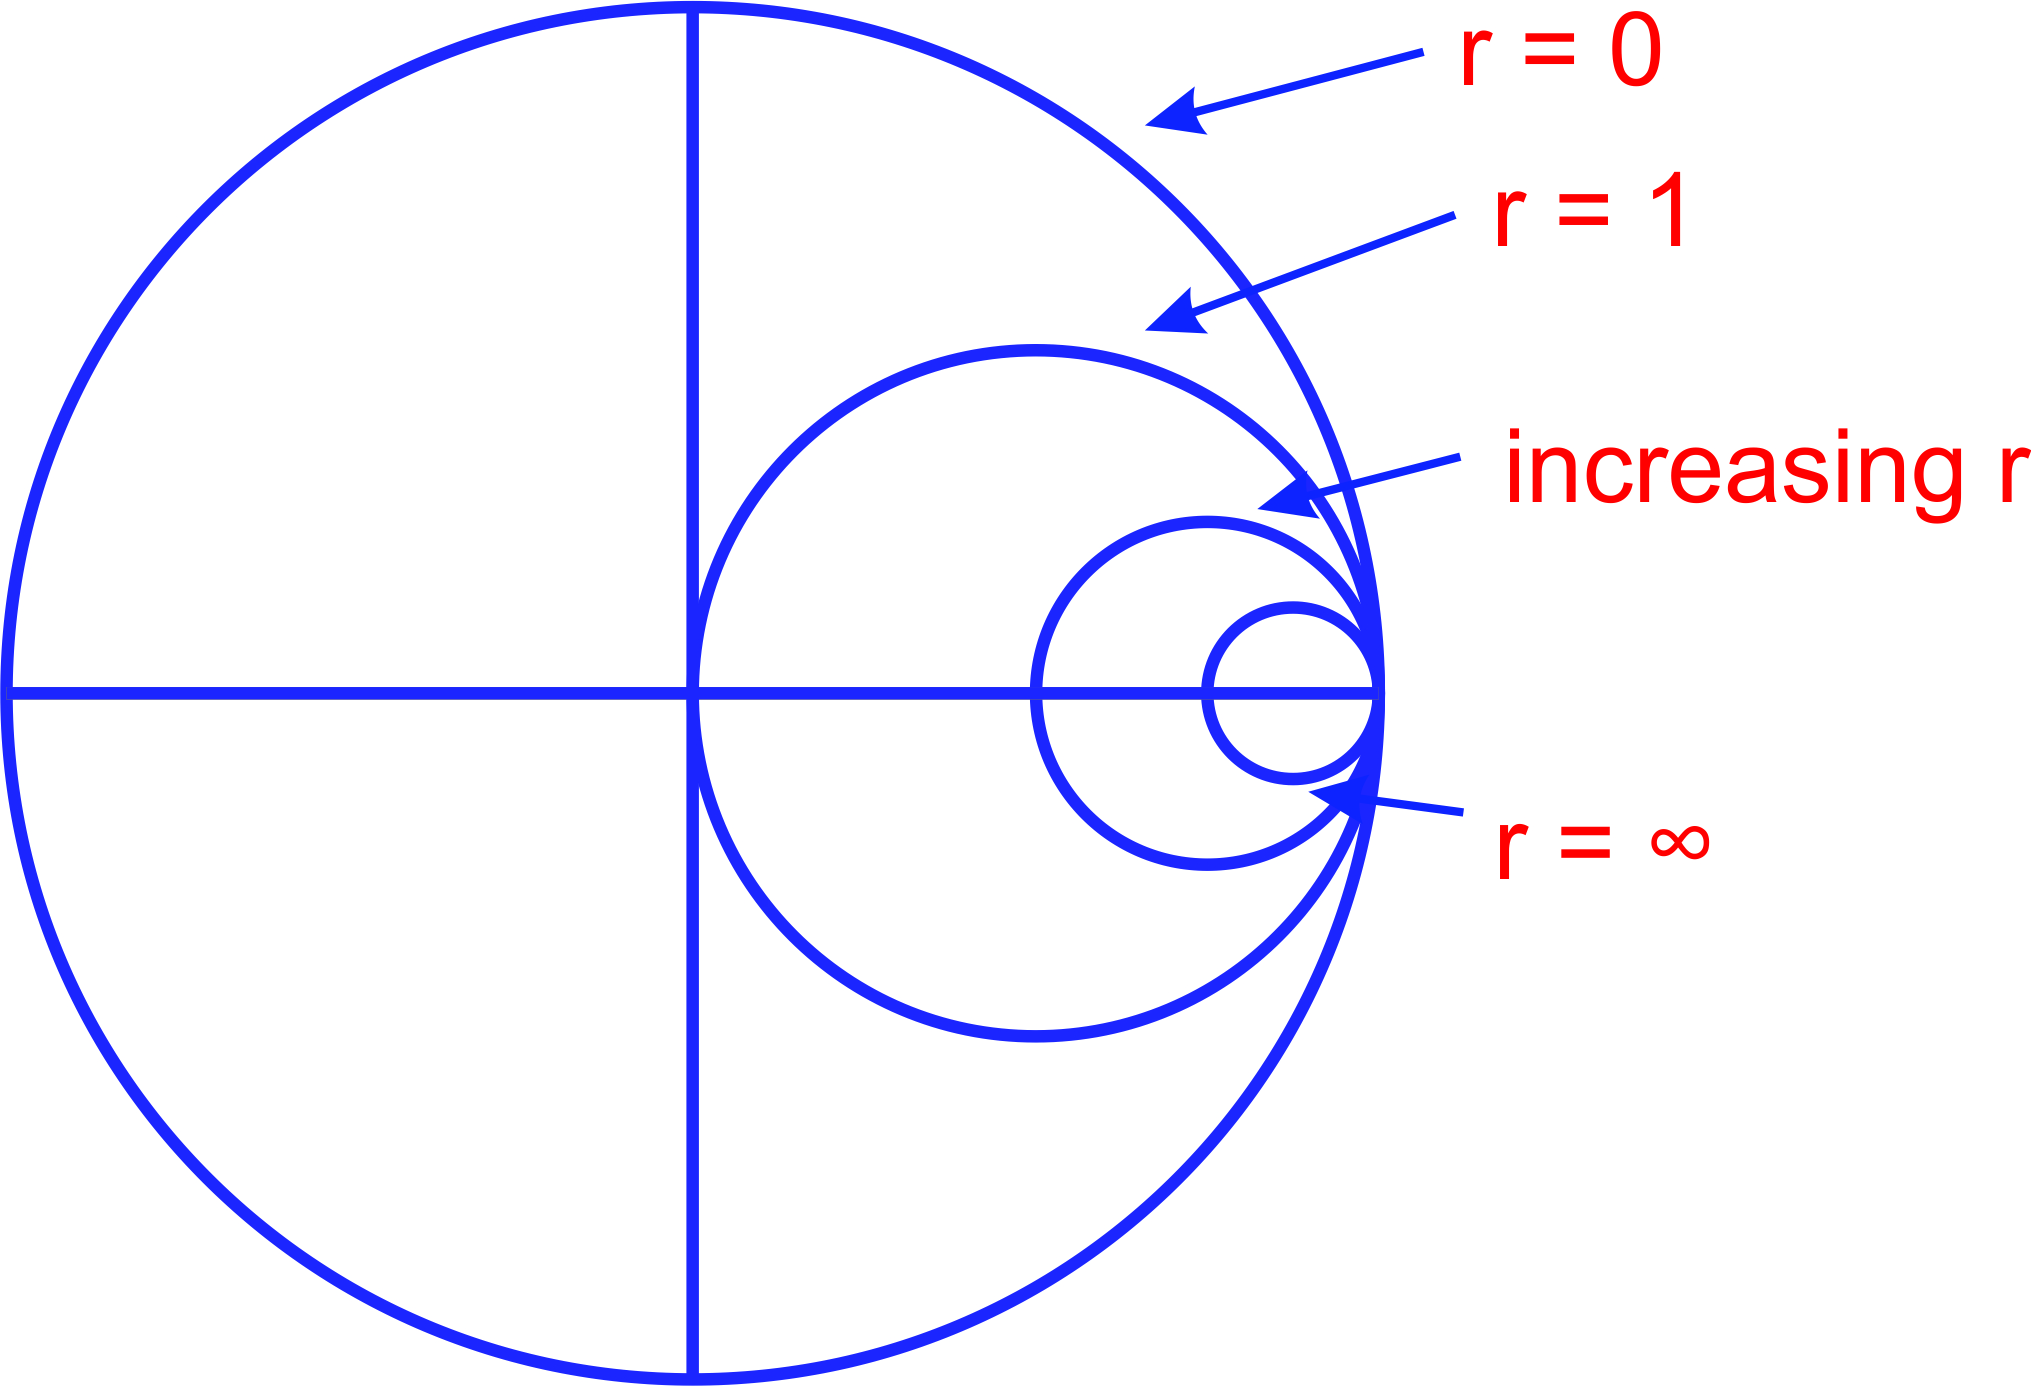
\includegraphics[width=0.5\linewidth]{./graphics/rghmgfcx}
\caption{Circle of Increasing Resistance}
\label{fig:rghmgfcx}
\end{figure}
We observe that all circle of the constant resistance circles passes through u = 1, and v = 0\\
Complex $\Gamma$ plane, Constant x circle where center is $(1,\frac{1}{x})$, and radius = $\frac{1}{x}$\\
For $x = \infty,Center = (1,0), radius = 0$\\
$x = 1,Center = (1,1), radius = 1$\\
$x = 2,Center = (1,\frac{1}{2}), radius = \frac{1}{2}$\\
\section{Circle of Constant Reactance}
\begin{align*}
u^2+v^2-2u\left(\frac{2}{x}\right)v+1=0
\end{align*}\\
Center = $(1,\frac{1}{x})$ and radius = $\frac{1}{x}$. \\
The centre of this circle lies on a vertical plane passing through the real axis at u=1 and the radius varies from $-\infty$ to $+\infty$.\\\\
From the plot above, it can be deduced that the centre always lie on a line u = 1 and v = 0. As x increases, the centre comes down along u = 1 line and the radius decreases.  
From the two plots above it is seen that both circles of constant resistance and reactance pass through co-ordinate (u,v) = (1,0). This signifies the uniqueness of the points.  When these two circles are superimposed, we have figure it as shown in figure~\ref{fig:uytrdbn}.
\begin{figure}[h]
\centering
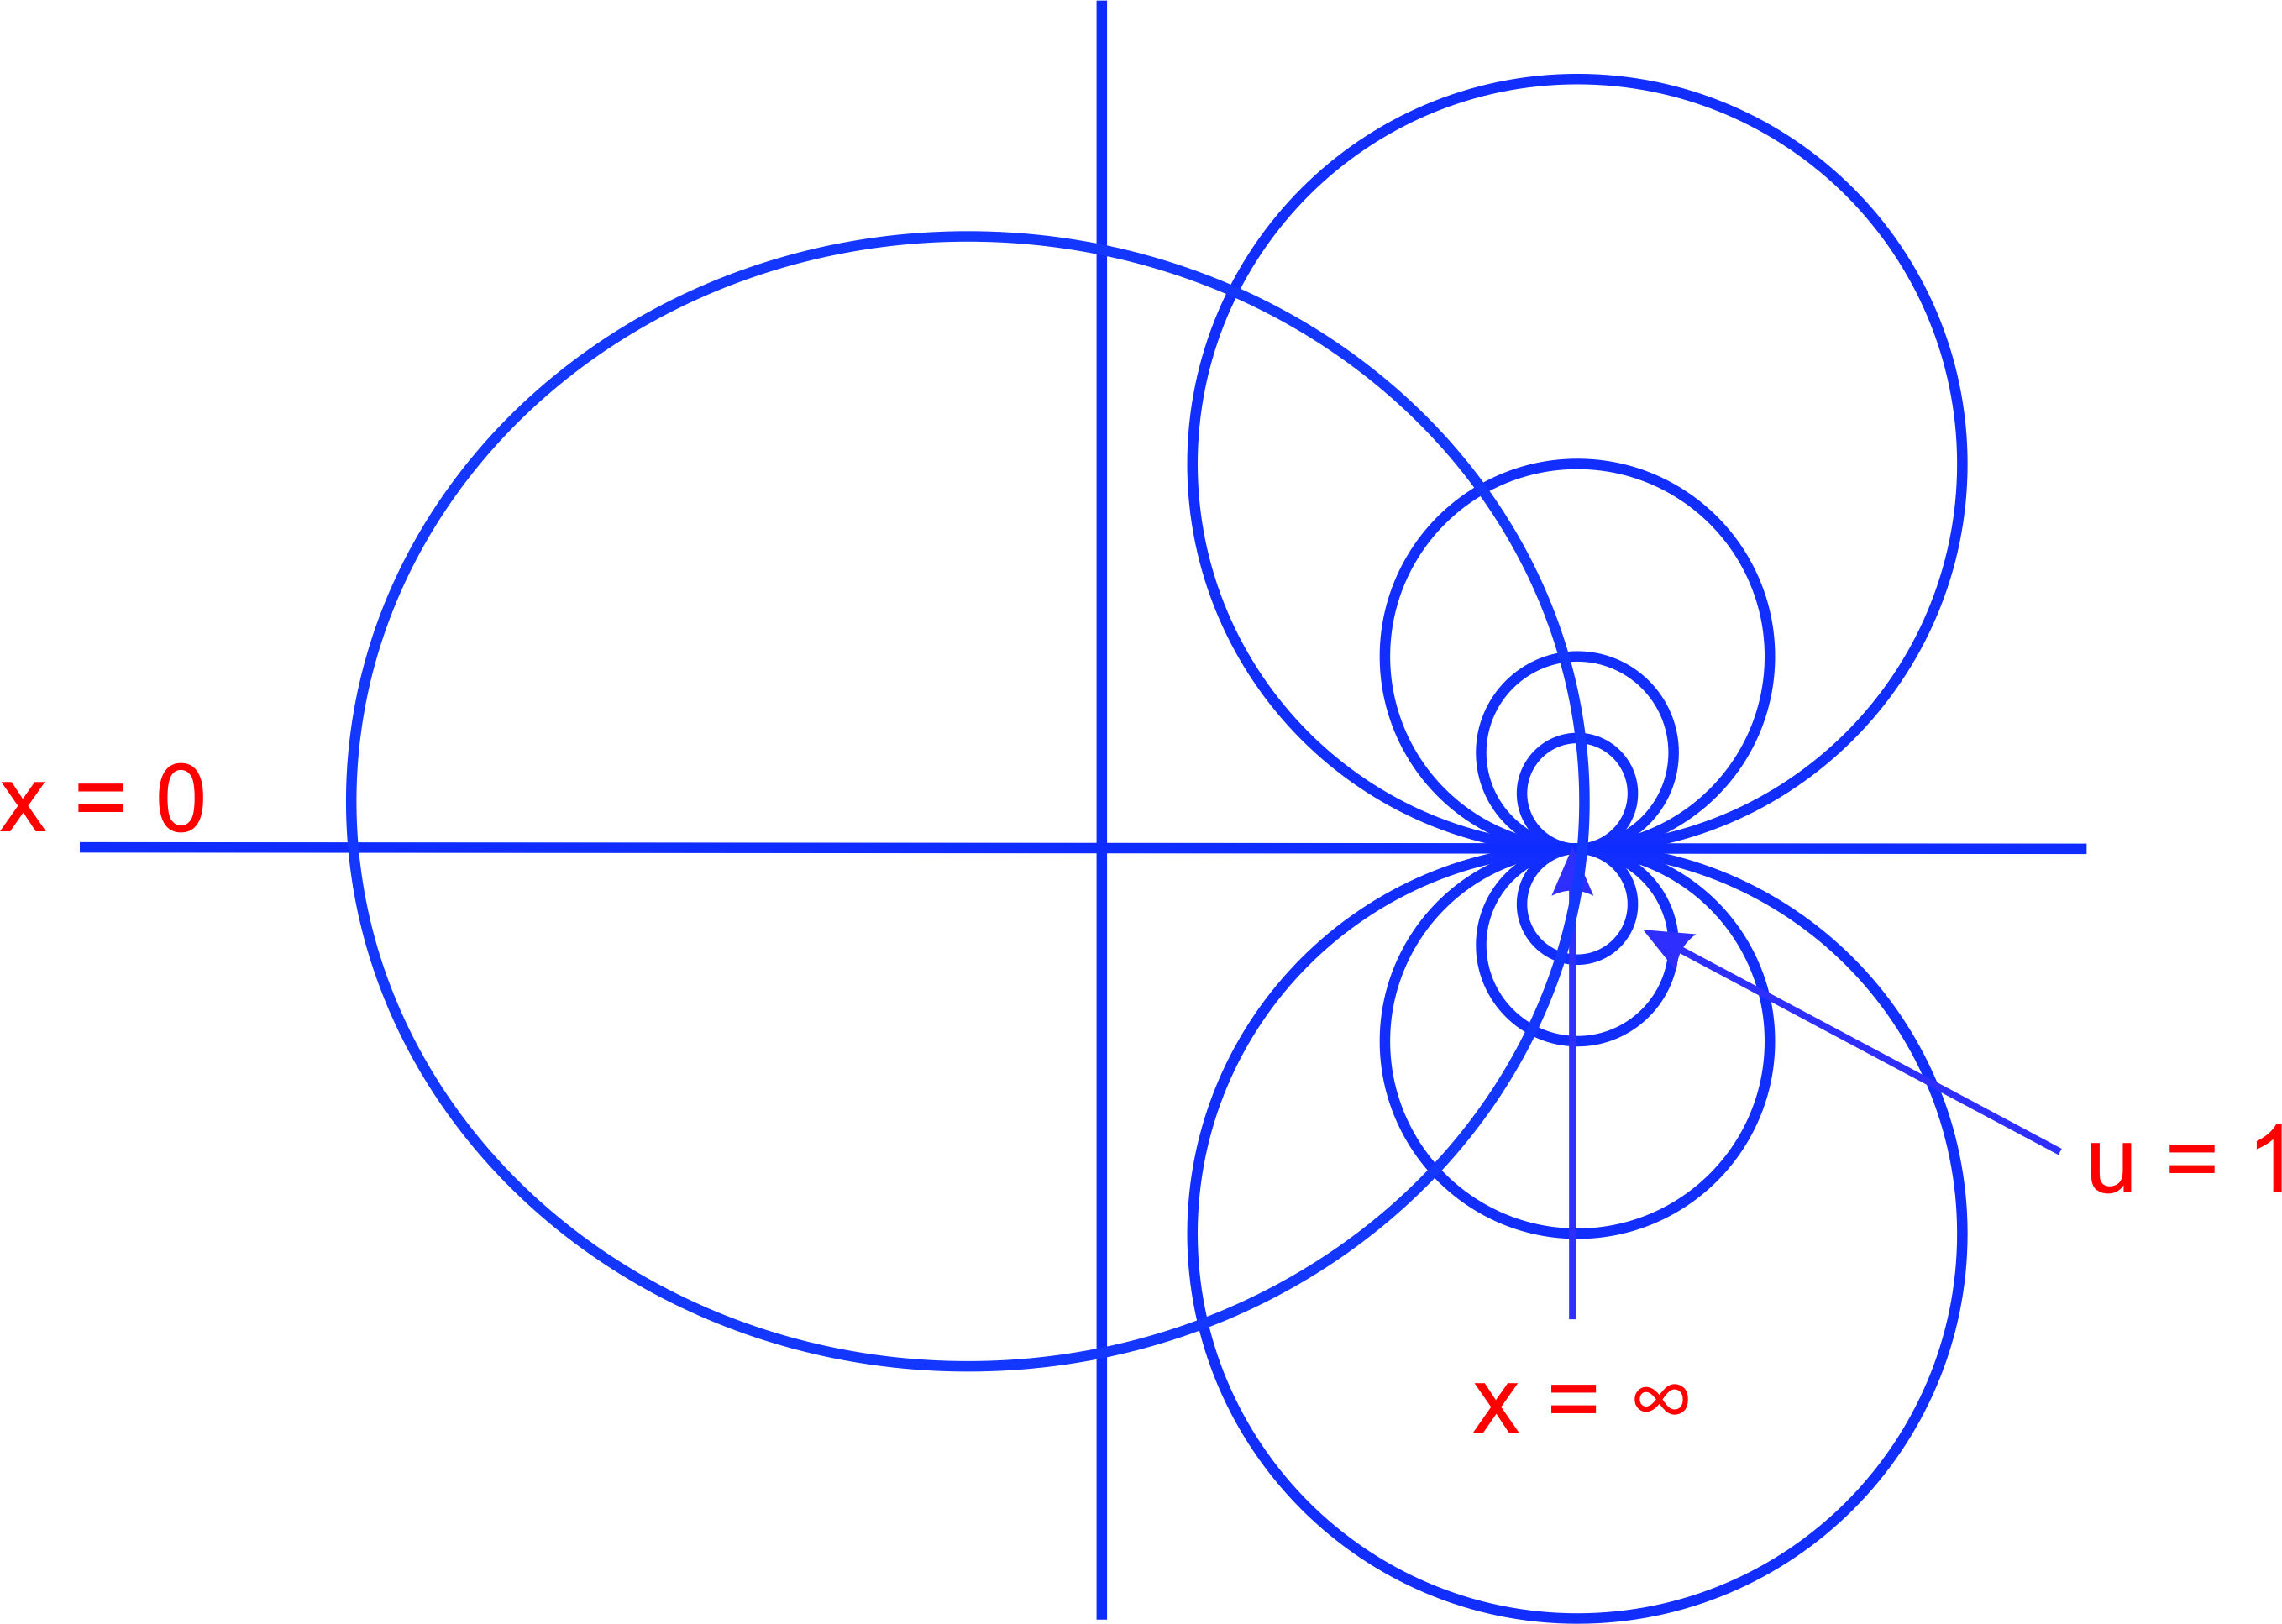
\includegraphics[width=0.5\linewidth]{./graphics/uytrdbn}
\caption{Two Set of Circles Superimposed}
\label{fig:uytrdbn}
\end{figure}

we observe that all circles of constant reactance also pass through (u,v) = (1,0). So the (u,v) = (1,0) is a special point as both constant resistance and reactance circle passes through that point. For the constant reactance circle, x = 0 gives the center $(1,\infty)$ and radius $\infty$. 

In this lecture, we are not concerned with reflection co-efficients that are greater than one, we are only interested in reflection co-efficient that are less than or equal to 1 which is represented by a unit circle of radius = 1. It therefore means that any other point outside this range of reflection co-efficient ($\Gamma$) is not of practical relevance to us since it does not represent a passive load.  Although, the constant reactance circle fills the entire space, but only the portion that satisfies $ \Gamma\ \leq 1$ is practically useful to us and this lies within the unit circle of the complex gamma plane.
\begin{figure}[h]
\centering
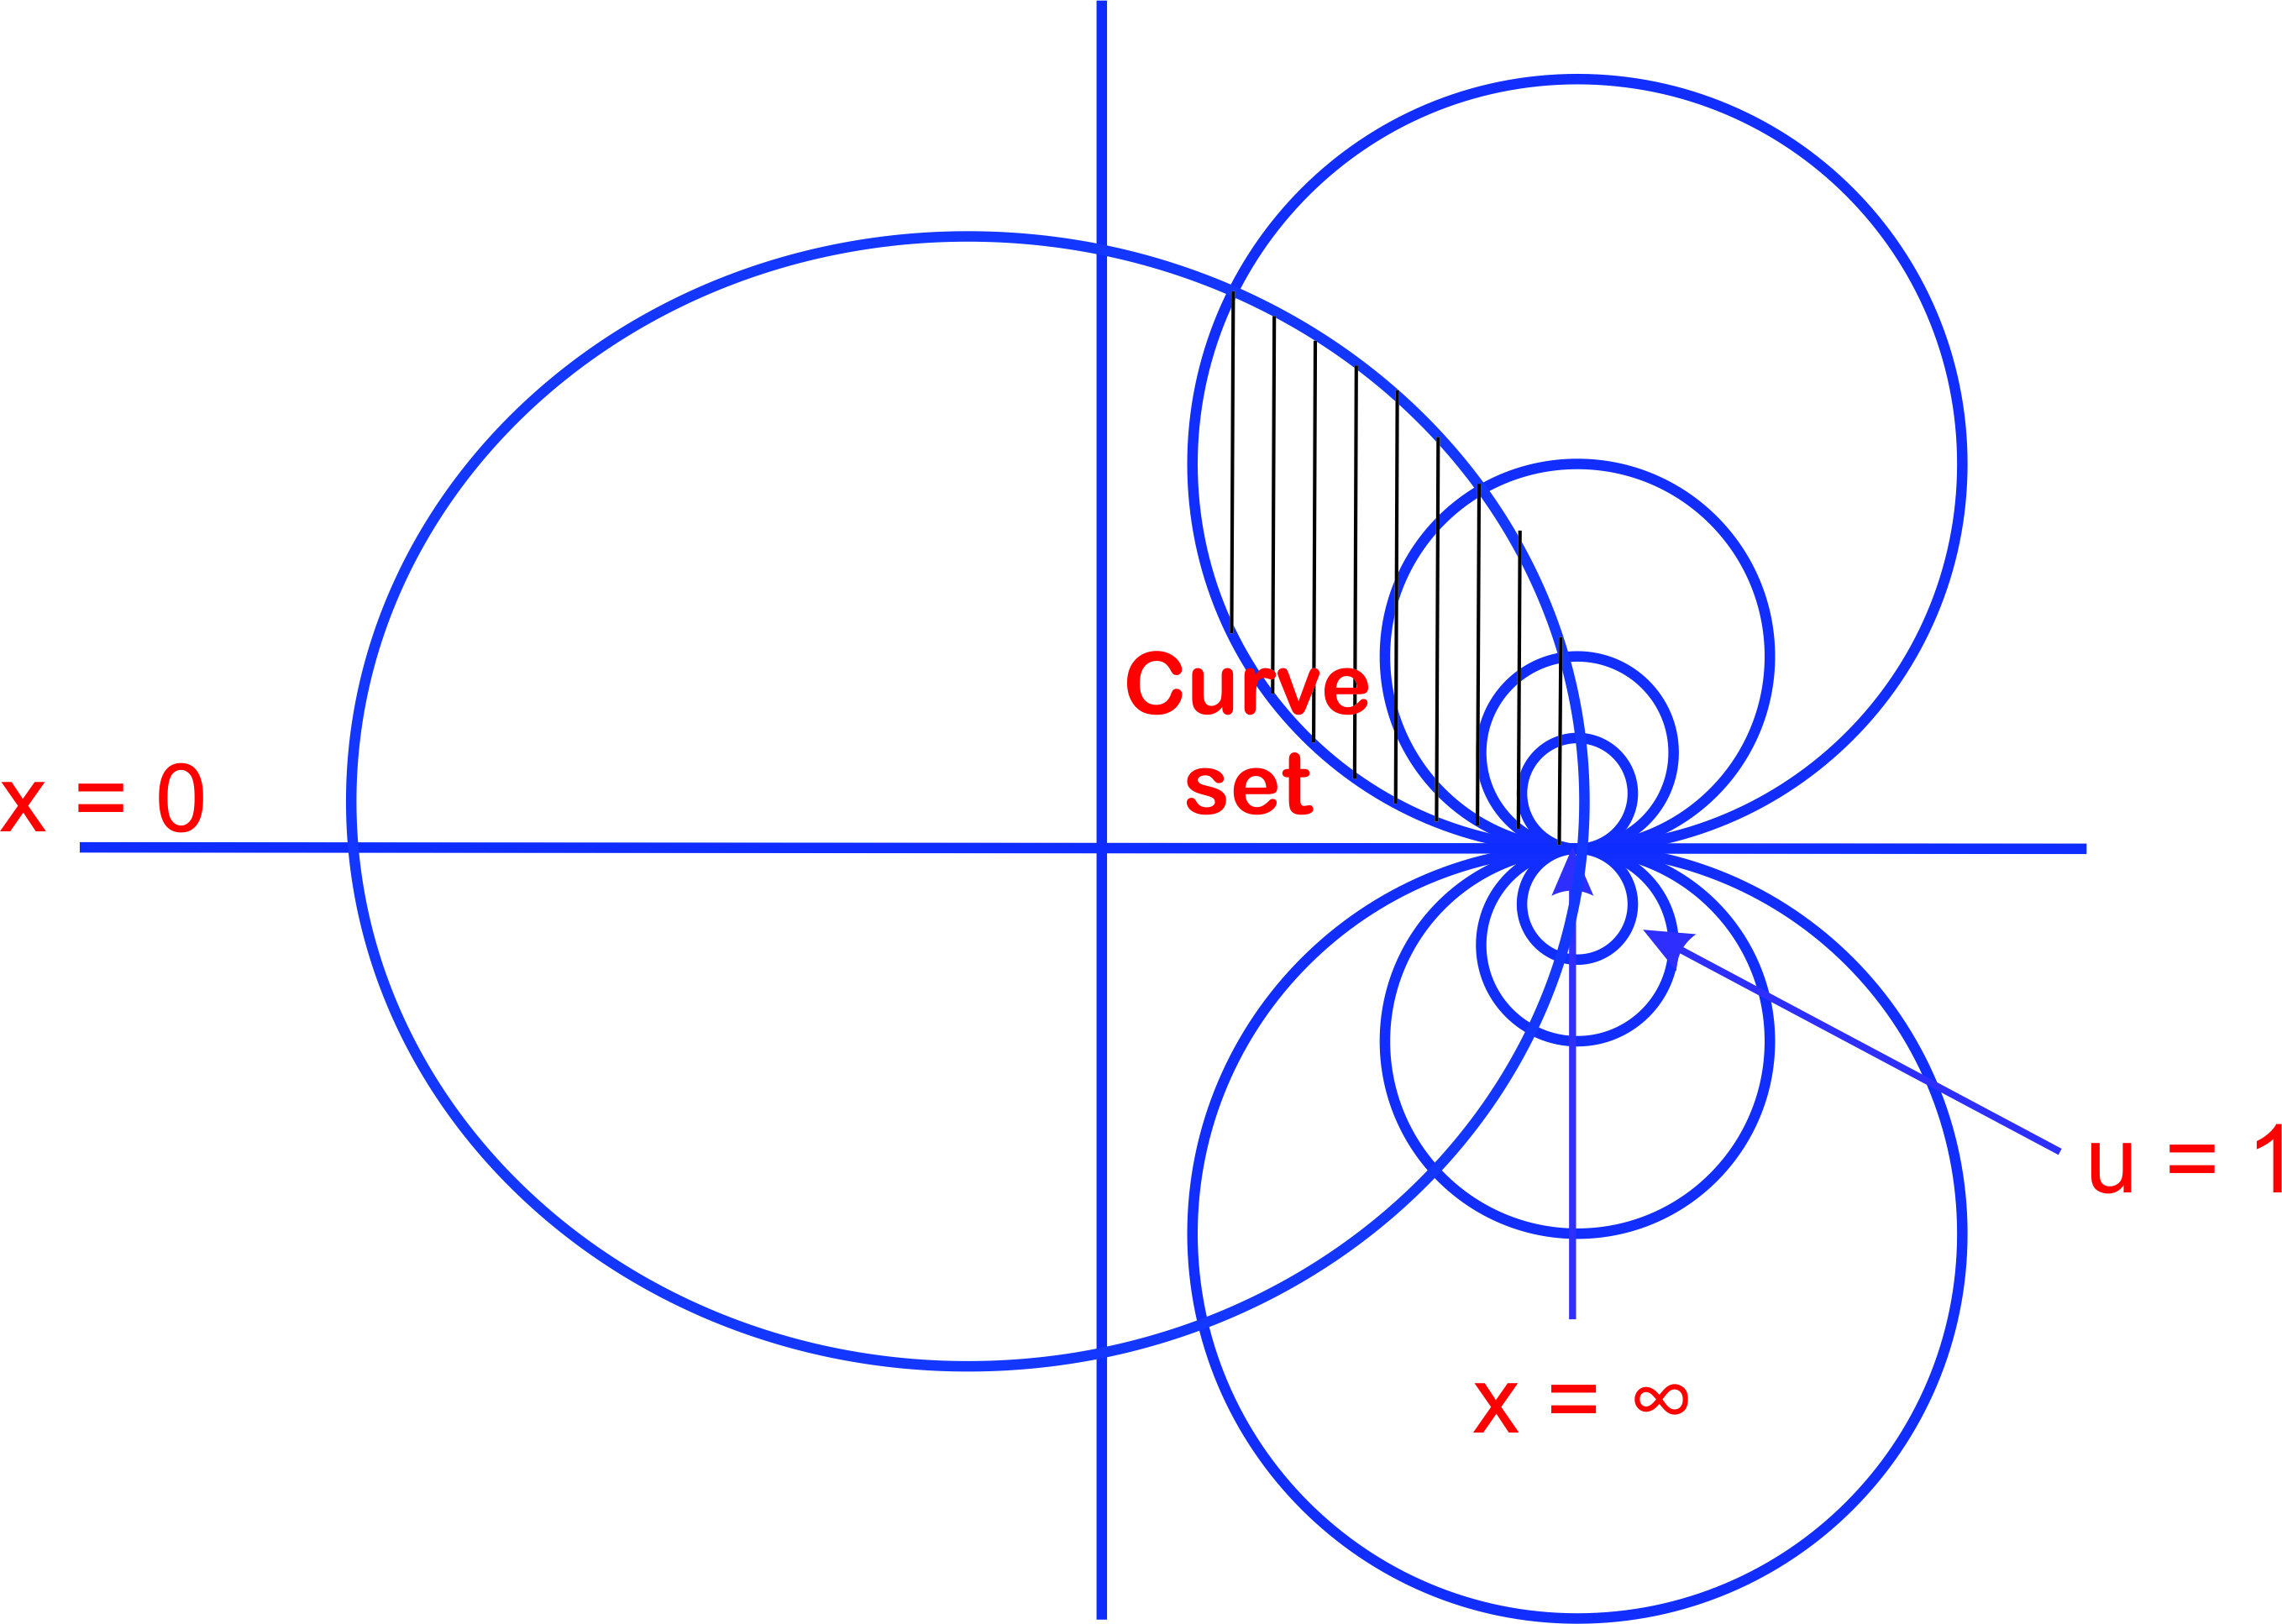
\includegraphics[width=0.5\linewidth]{./graphics/ijnbvcxw}
\caption{Two Set of Circles Superimposed}
\label{fig:ijnbvcxw}
\end{figure}
\begin{figure}[h]
\centering
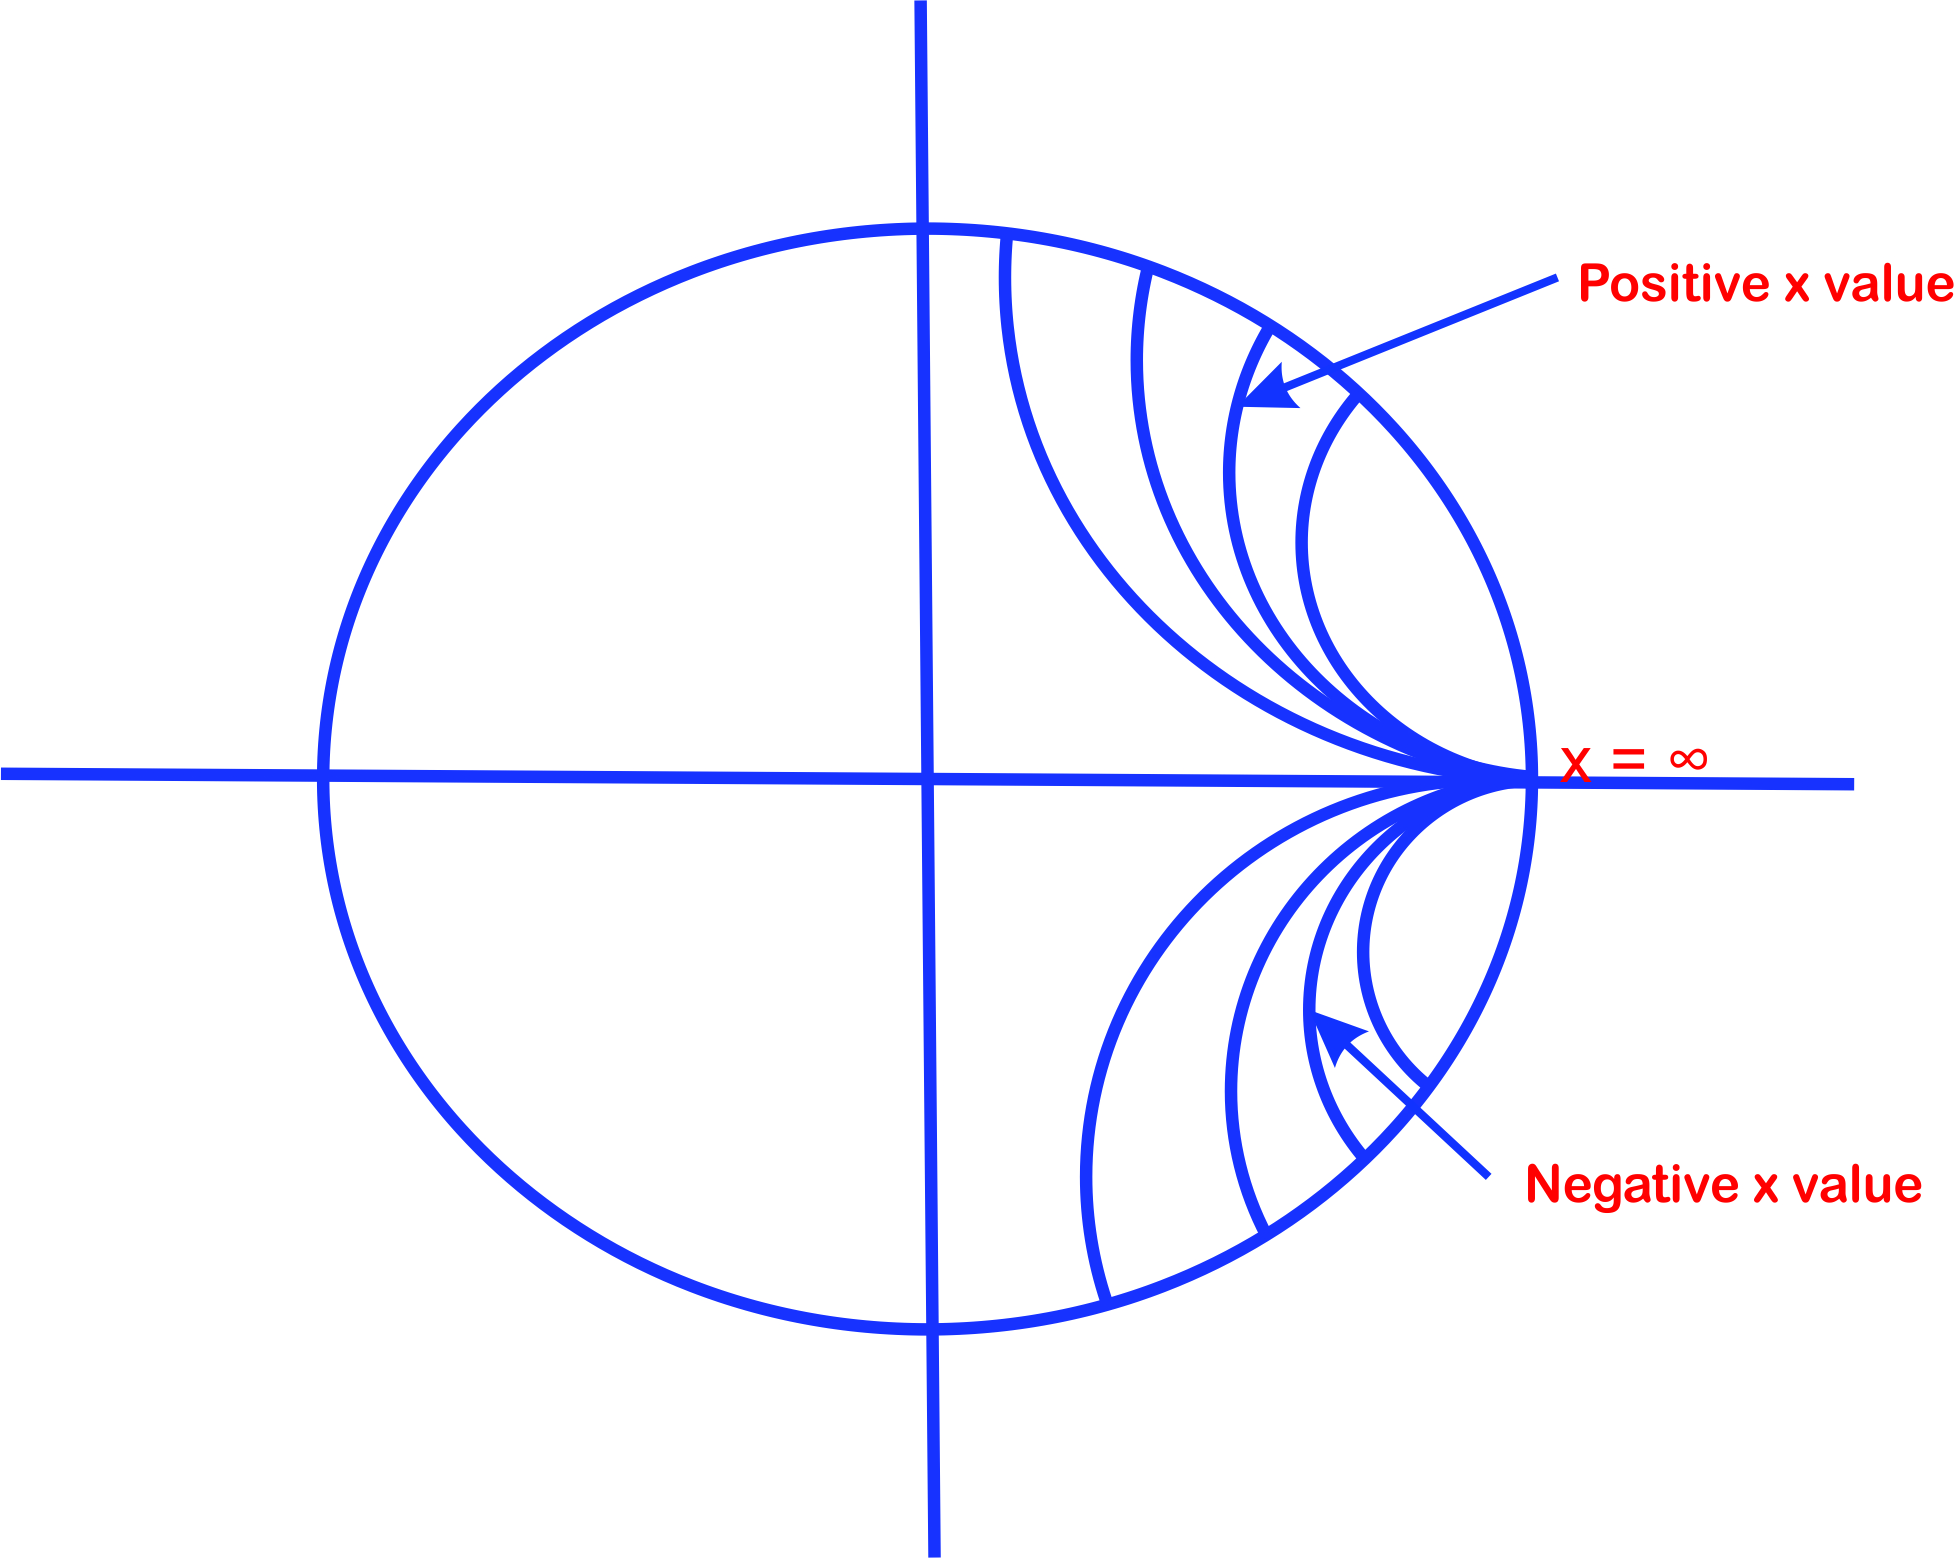
\includegraphics[width=0.5\linewidth]{./graphics/sddfghj}
\caption{Useful part of the Two Superimposed Circles}
\label{fig:sddfghj}
\end{figure}

This figure above is a superposition of constant resistance and reactance circles so, we can now identify the impedance point on the gamma plane.  The outermost circle of radius, $r= 1$, is called the limit circle for the gamma plane for which $\Gamma\ \leq 1$.\\

Some of the observations we made are summarized as follows:
\begin{enumerate}[(i)]
\item All constant resistance circles have their centre lying on the positive axis and complex gamma plane.
\item All the circles passes through the point u=1, v = 0
\item As the value of r increases, the centre shift towards the right from the origin to point u = 1 and the radius decreases.
\item The constant reactance circle has a vertical line passing through u=1 and the upper half represents the positive reactance and the lower half negative reactance.
\item As the reactance value increases, the centre of the circle approaches the u-axis, the radius of the circle decreases and the size of the circle reduces.
\item When x = $\infty$, the size of the circle = 0  and this  becomes just a point at (u,v) = (1,0).
\end{enumerate}

\section{The Smith Chart}
\begin{figure}[h]
\centering
\includegraphics[width=0.7\linewidth]{"./graphics/smith_chart (2)"}
\caption{A Complete Smith Chart}
\label{fig:smithchart-2}
\end{figure}

\footnote{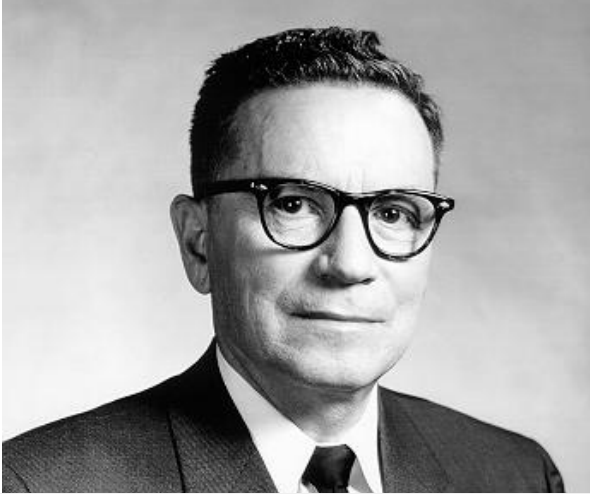
\includegraphics[scale=0.09]{./graphics/a21}PHILIP HAGAR SMITH (April 29, 1905 - August 29, 1987) was an electrical engineer who became famous for his invention of the SMITH CHART. He graduated from Tufts College in 1928 with a BS degree in electrical engineering while working for Bell Telephone Laboratories. He invented his eponymous smith chart during the period of being faced with the challenge of how to show and evaluate multiple complex impedance parameters which can range from zero to infinity. When asked why he invented the chart, Smith explained \textquotedblleft From the time I could operate a slide rule, I've been interested in graphical representations of mathematical relationship\textquotedblright. This interest in representing mathematical relationships in graphical form is what led to the invention of the smith chart.}

The smith chart is a graphical aid designed for electrical and electronics engineers to assist in solving problems of the transmission lines and matching circuits. It is a product of superimposing the circle of constant resistance and the circle of constant reactance. It can be used to simultaneously display multiple parameters such as the impedances, admittances, reflection co-efficient e.t.c.
It is plotted on the complex reflection co-efficient plane in two dimensions and is scaled in normalized impedance (which is most common), normalized admittance or both. It has circumstantial scaling of wavelengths and degrees. The wavelengths scale is used in distributed component problems and represents the distance measured along the transmission line connected between the generator and the load to the point under consideration.
Let us mark out some important points on the simplified smith chart below.
\begin{figure}[h]
\centering
\includegraphics[width=0.5\linewidth]{"./graphics/473 drawingjhgfd"}
\caption{A Simplified Smith Chart}
\label{fig:473-drawingjhgfd}
\end{figure}

\begin{enumerate}[(i)]
\item The point A or any other point lying on the outermost circle correspond to r = 0 while any point lying on the horizontal axis represents x = 0
\item The intersection of this horizontal axis and the outermost circle corresponds to r = 0,x = 0 at A which corresponds to a load that is short circuited from the impedance point of the line. It therefore means that point A is a short circuit.
\item At point B where the two set of circles degenerate into, corresponds to $r=\infty$ and $x=\infty$ which is nothing but an open circuit.\item Any point between A and B on the outermost circle represents pure reactance. Above the u axis inside the limit circle , we have the inductive loads while below the u axis in the limit circle we have the capacitive load( it therefore means we can tell what kind of load we have by where it lies on the smith chart).
\item At point C where r = 0 and x = +1, corresponds to purely inductive reactance whose magnitude is equal to the characteristic impedance of the line.
\item At point D where r = -1 and x = -1 represents a purely capacitive reactance whose magnitude is equal to the characteristic impedance of the line.
\item The centre of the limit circle has one more special point M which is the origin, it is the intersection of r = 1 circle and x = 0 line.

At M the impedance equal to the characteristic impedance of the line and that is the point of greatest interest to us because that point represents the matched condition of the transmission line.
\end{enumerate}
These points if properly understood can be used to solve transmission line problems with ease.

To solve transmission line problems using the smith chart, it should be held such that the most clustered portion of the circle should be held with the right hand of the user because the real axis at the complex gamma plane is in that direction and the complex imaginary plane is in the vertical direction.

With this understanding,
\begin{enumerate}[(i)]
\item Calculation on conversion from the complex reflection co-efficient plane to the impedance plane and vice versa can be done easily.
\item Impedance points on the smith chart can be marked and used to find co-ordinates of the point which gives the reflection co-efficient easily.
\end{enumerate}
The smith chart is a handy tool for solving very complex impedance transformation problems.
